
\chapter{Vorgehensweise}

\section{Inferenz der Pose des Agenten}

\subsection{Datengewinnung}

Zur Erzeugung der Trainingsdaten wird in jedem \texttt{step}-Aufruf des Simulators das dazugehörige Kamerabild der DuckieBots abgegriffen, mit dem korrespondierenden Label versehen und anschließend abgespeichert. Das Label beinhaltet hierbei folgende Informationen:

\begin{enumerate}
	\item Kürzester Abstand $d$ zur rechten Fahrbahnmarkierung
	\item Winkeldifferenz $\Theta$ zwischen Orientierung des DuckieBots und der Fahrbahn
	\item Name der Kachelart, auf der sich der DuckieBot zur Zeit der Aufnahme des Kamerabildes befindet
\end{enumerate}

Es kann außerdem gesteuert werden, wie viele Kamerabilder aufgenommen werden sollen.
Im folgenden werden wir auf zwei verschiedene Ansätze eingehen, die wir zur Gewinnung der Daten verfolgt haben:

\subsubsection{Ansatz 1 - PID-Fahrt ohne Neuplatzierung des Agenten:}

Der DuckieBot wird mittels eines PID-Reglers gesteuert, so dass er die Mitte der rechten Fahrspur hält und den Streckenverlauf der Fahrbahn verfolgt. Dabei wird der DuckieBot auf einer zufälligen befahrbaren Kachel der Umgebung platziert. Die Orientierung des DuckieBots  wird hierbei ebenfalls zufällig ausgewählt.

\subsubsection{Ansatz 2 - PID-Fahrt mit Neuplatzierungen des Agenten:}

Bei diesem Ansatz wird der DuckieBot ebenfalls mit Hilfe eines PID-Reglers (wie in Anstatz 1 beschrieben) gesteuert. Der Unterschied hierbei ist, dass der DuckieBot nach einer gewissen Anzahl von \texttt{step}-Aufrufen des Simulators neu platziert wird. Die Platzierung des DuckieBots erfolgt hierbei ebenfalls zufällig, nach dem im Ansatz 1 beschriebenen Verfahren. 

\subsection{Netzwerkarchitektur}

Unsere Netzwerkarchitektur besteht aus neun Schichten: einer Normalisierungsschicht, fünf Faltunsschichten und drei Fully-Connected-Schichten. Das Netzwerk nimmt das  Kamerabild des DuckieBots als Eingabe entgegen, wobei das obere drittel des Kamerabildes entfernt wurde. Dies hat den Vorteil, dass somit nur die relevanten Informationen für das Netzwerk im Kamerabild enthalten sind, wodurch sich das Training des Netzes verbessert. Das Netzwerk verarbeitet dann das eingehende Kamerabild und liefert anschließend die geschätze Pose, bestehend aus dem kürzestem Abstand $d$ zur rechten Fahrbahnmarkierung sowie der Winkeldifferenz $\Theta$ zwischen Orientierung des DuckieBots und der Fahrbahn.
Eine schematsche Darstellung der Netzarchitektur ist in Abbildung \ref{network-architecture} dargestellt. \\

Die Normalisierungsschicht des Netzwerks kümmert sich um die Normalisierung des Eingabebildes. Die Grundidee hinter dieser Schicht besteht darin, die Ausgabe einer Aktivierungsschicht zu normalisieren, wodurch die Konvergenz während des Trainingsprozesses verbessert wird. \cite{tensorflow} \\

Die Faltungsschichten kümmern sich um die Extraktion von Bildmerkmalen. Die ersten drei Faltungsschichten nutzen dabei einen 5x5 Kernel mit einer 2x2 Schrittbreite (stride) und die letzen beiden einen 3x3 Kernel mit einer 1x1-Schrittbreite. \\

Nach den Faltungsschichten folgen drei Fully-Connected-Schichten die uns schlussendlich die geschätzte Distanz $d$ und geschätzte Winkeldifferenz $\Theta$ liefern.


\begin{figure}[H]
	\centering
	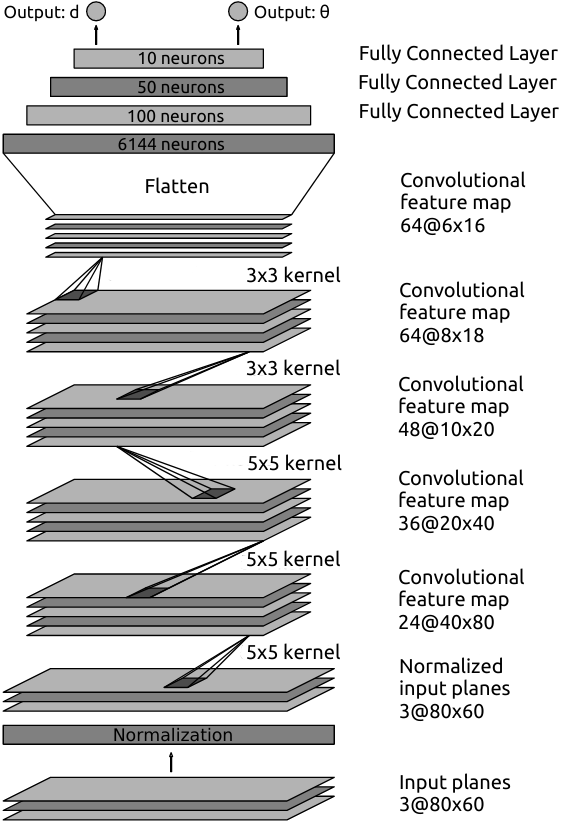
\includegraphics[width=0.75\textwidth]{kapitel4/images/network_architecture.png}
	\caption{Schematische Darstellung der Netzwerkarchitektur}
	\label{network-architecture}
	\vspace{0.2cm}
	\quelle\url{https://d3i71xaburhd42.cloudfront.net/0e3cc46583217ec81e87045a4f9ae3478a008227/5-Figure4-1.png}
\end{figure}

\section{Direkte Inferenz des Steuerbefehls}




